%%
%% ****** ljmsamp.tex 13.06.2018 ******
%%
\documentclass[
11pt,%
tightenlines,%
twoside,%
onecolumn,%
nofloats,%
nobibnotes,%
nofootinbib,%
superscriptaddress,%
noshowpacs,%
centertags]%
{revtex4}
\usepackage{ljm}
\begin{document}

\titlerunning{Application of machine learning elements} % for running heads
%\authorrunning{First-Author at al.} % for running heads
\authorrunning{Kosyakov, Legostaev} % for running heads

\title{Application of machine learning elements \\ to reconstruct the permeability and compressibility fields \\ of an oil reservoir development element}
% Splitting into lines is performed by the command \\
% The title is written in accordance with the rules of capitalization.

\author{\firstname{V.~P.}~\surname{Kosyakov}}
\email[E-mail: ]{lik.24@yandex.ru}
\affiliation{Tyumen Branch of Khristianovich Institute of Theoretical and Applied  Mechanics SB
	RAS, Taymirskaya ul. 74, 625026, Tyumen, Russia}


\author{\firstname{D. ~Yu.}~\surname{Legostaev}}
\email[E-mail: ]{legostaevdy@yandex.ru}
\affiliation{Tyumen Branch of Khristianovich Institute of Theoretical and Applied  Mechanics SB
	RAS, Taymirskaya ul. 74, 625026, Tyumen, Russia}
%\noaffiliation % If the author does not specify a place of work.

\firstcollaboration{(Submitted by ...)} % Add if you know submitter.
%\lastcollaboration{ }

\received{June 13, 2018} % The date of receipt to the editor, i.e. December 06, 2017


\begin{abstract} % You shouldn't use formulas and citations in the abstract.
In the oil industry, there is a noticeable trend towards using proxy models to simulate various levels of complexity in order to make operational predictions. In particular, machine learning techniques are being actively developed in the context of the digitalization and automation of production processes.
This paper presents an approach to combining a physically relevant fluid flow model with machine learning methods in order to address adaptation and prediction challenges. The approach is demonstrated through the use of synthetic oil reservoir models.
A feature of the considered synthetic model is the presence of a pronounced zonal inhomogeneity of the permeability field. 
Within the framework of the proposed approach, a single-phase filtration model, simplified in comparison with the original formulation, was used, which was history-matched by restoring the field of reservoir filtration parameters using a network of radial basis functions. Based on the reconstructed field, the connection coefficients between the wells were calculated, which qualitatively and quantitatively correspond to the true well connection. The next step was to train the recurrent neural network in order to predict the water cut of the produced fluid. The use of a recurrent neural network made it possible to reproduce the characteristic non-monotonic behavior of the water cut of the produced fluid, caused by non-stationary modes of operation of injection and production wells. A combination of the presented models makes it possible to predict the volume of the produced fluid and its phase composition. To assess the predictive properties of the models, the actual data set was divided into training and test intervals.
\end{abstract}

\subclass{76S05,90C31} % Enter 2010 Mathematics Subject Classification.

\keywords{flow through porous medium, reservoir mathematical simulation, inverse problem, adjoint problem, machine learning, radial basis functions} % Include keywords separeted by comma.

\maketitle

% Text of article starts here.

\section{Introduction}
Currently, in the oil industry, in addition to the use of traditional hydrodynamic models, the use of simplified proxy models has become widespread. This use of simplified modeling reduces computational costs and also reduces the requirements for the quality and completeness of source data. The development and application of proxy modeling in inverse and optimization problems are relevant, as these are the most resource-intensive tasks. Apart from physically meaningful models, such as material balance \cite{mus1}, super elements, CRM \cite{bek} and streamlines \cite{pot}, approaches based on machine learning techniques are also being explored  \cite{tem}, \cite{uma}. However, the use of machine learning-based techniques alone as predictive models cannot ensure that the results are accurate from a physical perspective. The combined use of physically meaningful models and machine learning techniques avoids these kinds of problems \cite{kos2}. The goal of this research is to develop proxy models that are based on the theory of fluid flow in porous media and machine learning principles. 

The figure \ref{fig:schime1} illustrates the general approach used in this work. The algorithm combines machine learning techniques (ML) with a physical model of single-phase fluid flow (Flow), which acts as one of the components in a "hybrid" neural network architecture. In this framework, some of the data from the "Input ML" is fed as input into the machine learning module. The output values from the machine learning process are then calculated and combined with the remaining data from the Input Flow to act as the input for the Flow calculations. To tune parameters in the machine learning model, we use the results from solving a similar problem, which enables us to compute gradients for the filtration process. Gradient calculations for the machine learning components are performed using the standard backpropagation error method.For the single-phase flow model, the gradient calculation is a separate and time-consuming process with a computational complexity that is typically comparable to or greater than that of direct calculations. The gradient calculation for the single-phase flow model is performed in a separate block when solving the conjugate problem.

\begin{figure}
	\centering
	\includegraphics[width=0.7\linewidth]{fig0}
	\caption{A calculation scheme for the proposed algorithm for the combined use of machine learning and a single-phase flow model.}
	\label{fig:schime1}
\end{figure}

The purpose of this research is to develop proxy models based on the theory of fluid flow through porous media and machine-learning techniques. The goal is to estimate hydroconductivity and capacitance parameters for reservoir systems in interwell spaces. This has been achieved using a fluid-flow model and known reservoir pressures at specific flow rates in the wells. To control predictive accuracy, the simulated production period was divided into a training interval and a test interval.

\section{Mathematical Model}

\subsection{Single-phase flow model}
To solve this problem, a two-dimensional mathematical model of single-phase flow of a
weakly compressible fluid was used as a filtration model \cite{bas}:

\begin{equation} \label{fil}
	\triangledown \cdot \left[\frac{k}{\mu}\triangledown P \right] = \beta \frac{\partial P}{\partial t} + \delta(x_1,x_2),
\end{equation}

\begin{equation} \label{bc}
	\delta(x_1,x_2)  = \left\{\begin{array}{crl}
		0, \;\mbox{if}\;(x_1,x_2) \notin\ \Gamma_{in}\cup\Gamma_{out},\\
		q_{i}, \;\mbox{if}\;(x_1,x_2) \in \Gamma_{in},\\
		q_{a}, \;\mbox{if}\;(x_1,x_2) \in \Gamma_{out},
	\end{array}\right. 
\end{equation}
Closing ratios:
\begin{equation} \label{kr}
	P = P_0\mbox{,\quad \mbox{if} $t=0$},
\end{equation}
where $k$ is permeability, $P$ is reservoir pressure, $\beta$ is
effective compressibility, $q_i$ is fluid flow rate in $i$-th well, $\Gamma_{in}$
is set of coordinates of sources/drain (wells), $\Gamma_{out}$ is
outer boundary, $P_0$ is reservoir pressure at the initial time $t=0$, $x_1$ and $x_2$ are coordinates, $q_{a}$ is specific fluid flow rate through the outer boundary, which can be written as:
\begin{equation*} \label{qaq}
	q_{a} = T_{a}(P_{a} - P|_{\Gamma_{out}}),
\end{equation*}
where $P_a$ is on the aquifer ($P_a = P_0$), $T_a$ is
aquifer boundary transmissibility (includes aquifer productivity factor). The goal of the inverse problem is to find the reservior permeability $k = k(x_1,x_2)$ and effective compressibility $\beta = \beta(x_1,x_2)$ at which the calculated values of reservoir pressure and water flow rate on the wells will satisfactorily coincide with the initial values.

\subsection{Single-phase flow model}

Obtaining the values of $k(x_1,x_2)$ and $\beta(x_1,x_2)$ can be done in various ways. For example, by interpolating and extrapolating measured values near the wells within the well space. This article suggests using a machine learning model to obtain the desired values. A two-layer neural network, consisting of a radial basis function (RBF) layer and a fully connected (linear) layer, was chosen as the machine learning model. The RBF layer determines the influence of each basis at a selected point in space.

When solving the inverse problem, it is more convenient to switch from permeability $k$ to general mobility $\lambda$. Using this parameter, it is possible to consider many filtration parameters that affect the flow structure (such as viscosity, relative phase permeability, and others). The fields of general mobility $\lambda$ and effective compressibility $\beta$ can be considered as functional dependences of $\lambda(\mathbf{x})$ and $\beta(\mathbf{x})$, where $\mathbf{x} = (x_1,x_2)$ is a vector of spatial coordinates, and a network of radially basis functions is used for the dependency.


\begin{eqnarray}\label{rbf}
	f_i(\mathbf{x}) = exp \left(\frac{-\lVert \mathbf{x} - \mathbf{c_f}_i \rVert^2}{\epsilon_{fi}^2}\right), \quad
	g_i(\mathbf{x}) = exp \left(\frac{-\lVert \mathbf{x} - \mathbf{c_g}_i \rVert^2}{\epsilon_{gi}^2}\right),
\end{eqnarray}

\begin{eqnarray*}
	\lambda(\mathbf{x}) = w_{fi}f_i + b_h, \quad
	\beta(\mathbf{x}) = w_{gi}g_i + b_g,
\end{eqnarray*}
where $\mathbf{x}$ are the coordinates of the calculated nodes, $\mathbf{c_f}_i$ and $\mathbf{c_g}_i$ are the position of the bases, $\epsilon_{fi}$ and $\epsilon_{gi}$ are the width of the bases, $w_{fi}$ and $w_{gi}$ are the weights of the bases, $b_f$ and $b_g$ are the free term. The parameters of the network of radial basis functions $\mathbf{c}_i$, $\epsilon_i$, $w_i$, $b$ are adjusted during the matching of the single-phase flow model.

\subsection{Inverse problem}


The inverse problem can be solved using an optimization approach that involves minimizing the objective function $J$.
The objective function can be expressed as the sum of terms, each term being the product of a function that characterizes the deviation of the calculated values from the target values, and a corresponding weighting factor. Standard error was used as a measure of deviation (MSE):
\begin{equation} \label{mse}
	J=\frac{w_p}{N_p}\sum_{i=1}^{N_p}{\left(p_c^i-p_f^i\right)^2}+
	\frac{w_{\lambda}}{N_\lambda}\sum_{i=1}^{N_\lambda}{\left(\Delta\lambda^i  \right)^2}+
	\frac{w_{\beta}}{N_\beta}\sum_{i=1}^{N_\beta}{\left(\Delta\beta^i  \right)^2},
\end{equation}
\begin{equation} \label{mse1}
	\Delta\lambda^i  = \left\{\begin{array}{crl}
		\lambda^i_c - \lambda^i_r, \quad \;\mbox{if}\; \lambda^i_c \ge \lambda^i_r\\
		0,\quad \;\mbox{if}\; \lambda^i_l < \lambda^i_c < \lambda^i_r\\
		\lambda^i_c - \lambda^i_l, \quad \;\mbox{if}\;\lambda^i_c \le \lambda^i_l
	\end{array}\right.,
	\quad
	\Delta\beta^i  = \left\{\begin{array}{crl}
		\beta^i_c - \beta^i_r, \quad \;\mbox{if}\; \beta^i \ge \beta^i_r\\
		0,\quad \;\mbox{if}\; \beta^i_l < \beta^i_c < \beta^i_r\\
		\beta^i_c - \beta^i_l, \quad \;\mbox{if}\;\beta^i_c \le \beta^i_l,
	\end{array}\right.
\end{equation}	
where $p_c^i$ is the calculated value of reservoir pressure, $p_f^i$
is the true value, $i$ is the measurement number, $N_p$ is the
number of reservoir pressure measurements,$N_\lambda$ is the
number of known mobility values and $N_\beta$ is the number of known values of effective compressibility, $\lambda$ is the true value of mobility near the welll, $\lambda_c$ is the calculated value of mobility, $\lambda_l$ and $\lambda_r$ are the left and right restrictions on the value of total mobility, $\beta$ is the true value of the elastic capacity near the well. $\beta_c$ is the estimated value of elasticity, $\beta_{l}$ and $\beta{r}$ represent the left and right limits on the elasticity range.

The second and third terms in the objective function ({\ref{mse}})--({\ref{mse1}}) are responsible for adjusting the mobility field and effective compressibility to match known values of the reservoir's filtration-capacitive properties. Furthermore, the calculated values for mobility and effective compressibility may vary within a range from $\lambda_l$ to $\lambda_r$ and from $\beta_l$ to $\beta_r$. However, this does not lead to an increase in the objective function, as long as the interval is acceptable. The presence of this interval is linked to changes in the phase composition of wells over time and their effect on the downhole mobility and compressibility.

The optimization problem is solved when each component of the gradient of the objective function tends to 0, which can be written as:
\begin{equation*}\label{grad}
	\frac{\partial J}{\partial u_k} = 
	2w_p\frac{1}{N}\sum_{i=1}^N	({p_c^i-p_f^i}) \frac{\partial p_c^i}{\partial u_k}+
	2w_{\lambda}\frac{1}{N_\lambda}\sum_{i=1}^{N_\lambda}{\Delta\lambda^i}\frac{\partial
		\lambda_{c}^i}{\partial u_k}+
	2w_{\beta}\frac{1}{N_\beta}\sum_{i=1}^{N_\beta}{\Delta\beta^i}\frac{\partial
		\beta_{c}^i}{\partial u_k}.
\end{equation*}
To solve the optimization problem, it is necessary that each
component  of the objective function gradient tends to 0, which can
be written as
\begin{equation} \label{rp}
	\frac{\partial J}{\partial u_k} \rightarrow 0.
\end{equation}

In order to solve the inverse problem using the gradient descent method, it is necessary to calculate the components of the gradient vector of the objective function, using configurable parameters. Parameters RBF (\ref{rbf}) can be used as these configurable parameters. Components of the gradient vector:

\begin{equation*}
	\frac{\partial J}{\partial w},\quad \frac{\partial J}{\partial \epsilon},\quad \frac{\partial J}{\partial b}, \quad \frac{\partial J}{\partial \mathbf{c}}.
\end{equation*}

Additional terms can be added to the target function (\ref{mse}), which are penalty functions that allow for regularization of the resulting solutions. A new term was added, which allows  to control the position of the basis functions (\ref{rbf}) relative to each other and the computational domain. If the basis functions are located close to each other or extend beyond the boundaries of the computational area, an additional penalty will be added to the target function.

\begin{equation} \label{pnl}
	J_{pnl}=\frac{2w_{dist}}{N_\textbf{x}*(N_\textbf{x}-1)}\sum_{i=1}^{N_\textbf{x}}{\sum_{j=i+1 }^{N_\textbf{x}}{\left(f_{relu}\left(r_{min} - r_{i,j}\right)\right)^2}} + 
	\frac{w_{bnd}}{N_\textbf{x}}\sum_{i=1}^{N_\textbf{x}}{\left(f_{relu}\left(r_{i,c} - \frac{L}{2}\right)\right)^2},
\end{equation}
where $w_{dist}$ and $w_{dist}$ are the weight coefficients for penalty functions in terms of the distance between the bases and the position relative to the boundaries of the calculated area, $N_\textbf{x}$ is the number of bases, $r_{i,j}$ is the distance between the $i$th and $j$th $r_{min}$ is the minimum allowable distance between the bases, $r_{i,c}$ is the distance from the i-th basis to the center of the calculated area, $f_{relu}$ is the activation function (rectified linear unit).

Gradients are computed using the standard machine learning technique of error backpropagation, which in this instance involves solving a conjugate problem for the single-phase flow model  \cite{kos3}, \cite{far}. This is done by solving for the derivative of the objective function with respect to physically meaningful parameters such as mobility and elastic capacity $\frac{\partial J}{\partial \lambda}$ and $\frac{\partial J}{\partial \beta}$. These derivatives are then used to calculate the gradients of the objective function, which are then passed to the machine learning algorithm. The Flux library \cite{inn}, written in the Julia programming language, was used to implement the presented approach, which allows for the calculation of gradients in a straightforward manner.


The solution of the inverse problem (\ref{rp}) is found  numerically
by the iterative method. At each iteration, the direct problem
(\ref{fil})--(\ref{kr}) is numerically solved and the derivatives of
the objective function are calculated according to the adjustable
parameters of the model. The numerical solution was found
by the control volume method for a two-dimensional rectangular
difference grid using the IMPES method \cite{azi}.

The objective function ({\ref{mse}}) used to solve the inverse problem is not always suitable for a subjective assessment of the accuracy of the model. Accuracy of the history-matching process was evaluated using the Mean Absolute Percentage Error (MAPE). This metric enables us to estimate the model's ability to accurately reproduce actual reservoir pressure, mobility values, and effective compressibility at wells.


\section{Results}

The proposed approach was tested using a synthetic model of an oil reservoir measuring 1000 x 1000 meters and 9 wells, 5 of these were producing wells (from P1 to P5), and 4 were injection wells (from I1 to I4). The model includes highly conductive inclusions with $k_1 = 1d$ and $k_2 = 0.5 d$, and the permeability in the main part of the region is $k = 0.1d$. Wells I3, I4 and P5 are located in an area where the effective compressibility is increased by 2 times.

\begin{figure}
	\centering
	
\includegraphics[width=0.7\linewidth]{fig1}
	\caption{Schematic representation of the computational domain}
	\label{fig:schime}
\end{figure}

To solve the inverse problem, fluid flow rates from producing and injection wells, obtained as a result of direct numerical modeling, were used as operating modes. Porosity, formation thickness, as well as initial and boundary conditions, corresponded to those in the direct problem.
The inverse problem is solved using an optimization formulation in which the objective function is minimized. This is achieved by summing the functions (\ref{mse}) and (\ref{pnl}).
When solving the problem, it was taken into consideration the possible lack of a complete dataset of reservoir pressure. In practice, only a limited number of pressure values are usually known, which rarely exceed 10-20\%. Consequently, of the results obtained by solving the direct problem, only 10\% of them were used as actual measurements of reservoir pressure, and the values were chosen at random. They served as true values in solving the inverse problem.

The simulation period lasted 10 years, during which time the wells operated according to the specified modes. The calculation step was 1 month. The time dependence of the injection rate of the injection wells, as shown in Fig. \ref{fig:inj_rate}, was obtained by random sampling and has a piecewise-constant form. Injection wells also shut down at a predetermined frequency. The downtime period ranged from 2 to 4 months. 
The time series show production from the wells Fig. \ref{fig:prod_rate}, was generated by randomly sampling values and has a piecewise-constant structure. The start of production wells was carried out in 3-month increments.
The resulting dataset was used to solve the inverse problem. In order to assess the predictive capabilities of the model, the data was divided into training and testing sets. The first seven years of development history were allocated to the training dataset and used to matching the model. The seven- to ten-year period was included in the test set for which forecasting calculations were carried out.

\begin{figure}
	\center{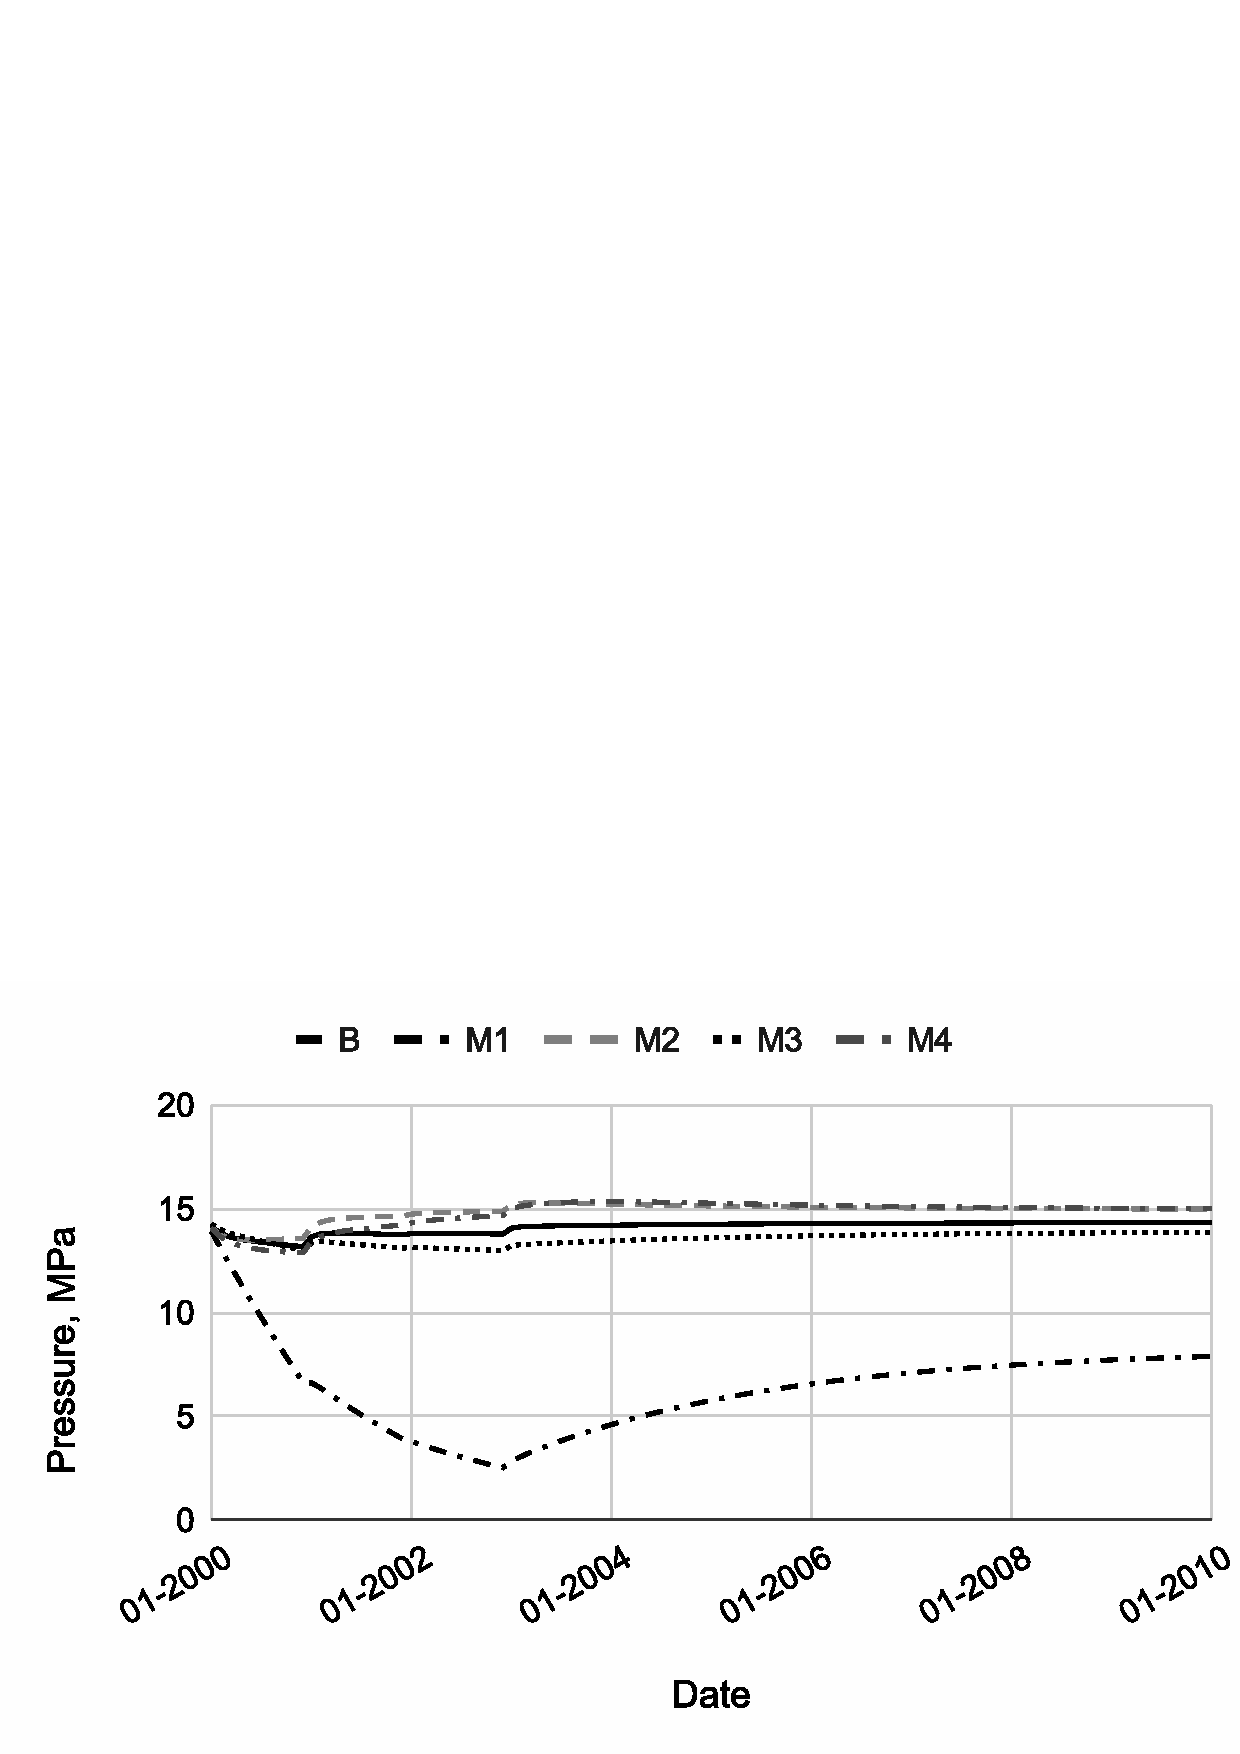
\includegraphics[height=0.40\linewidth]{fig2.png}}
	\caption{Injectivity dynamics of injection wells I1-I4}
	\label{fig:inj_rate}
\end{figure}

\begin{figure}
	\center{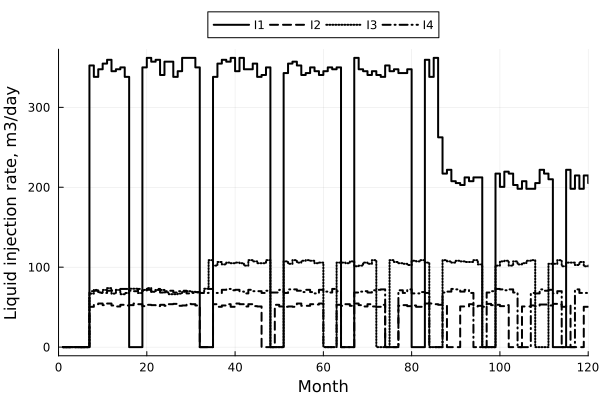
\includegraphics[height=0.40\linewidth]{fig3.png}}
	\caption{Productivity dynamics of production wells P1-P5}
	\label{fig:prod_rate}
\end{figure}

The initial reservoir pressure was set to $20 MPa$. At the boundaries of the development area, a constant reservoir pressure of $20 MPa$ was maintained. The parameters of the rock and fluid were as follows: porosity = $0.2$, absolute permeability, as shown in Fig. \ref{fig.:scheme}, effective viscosity = $1 Pa*s$, layer thickness = $4 m$, effective elastic capacity $10^{-4} MPa^{-1}$.

The optimization problem was solved using the optimization algorithms included in the Flux package (Descent and ADAM). As a result, mobility maps Fig. \ref{fig:mob} and maps of effective compressibility Fig. \ref{fig:comp} were obtained. Although there are differences, it can be seen that these fields qualitatively resemble the original ones \ref{fig:schime}. In addition to the mobility map, Table 1 presents the values of connections between wells. These were obtained by partially excluding variables from the numerical filtration model (And). The highest values for the I2-P1 and I3-P3 connections correspond to zones with high permeability (channels). The coupling coefficients make sense of conductivity between wells per unit thickness of formation. Similar values can be obtained through pairwise hydraulic monitoring of the wells.

\begin{figure}
	\begin{minipage}[h]{0.48\linewidth}
		\center{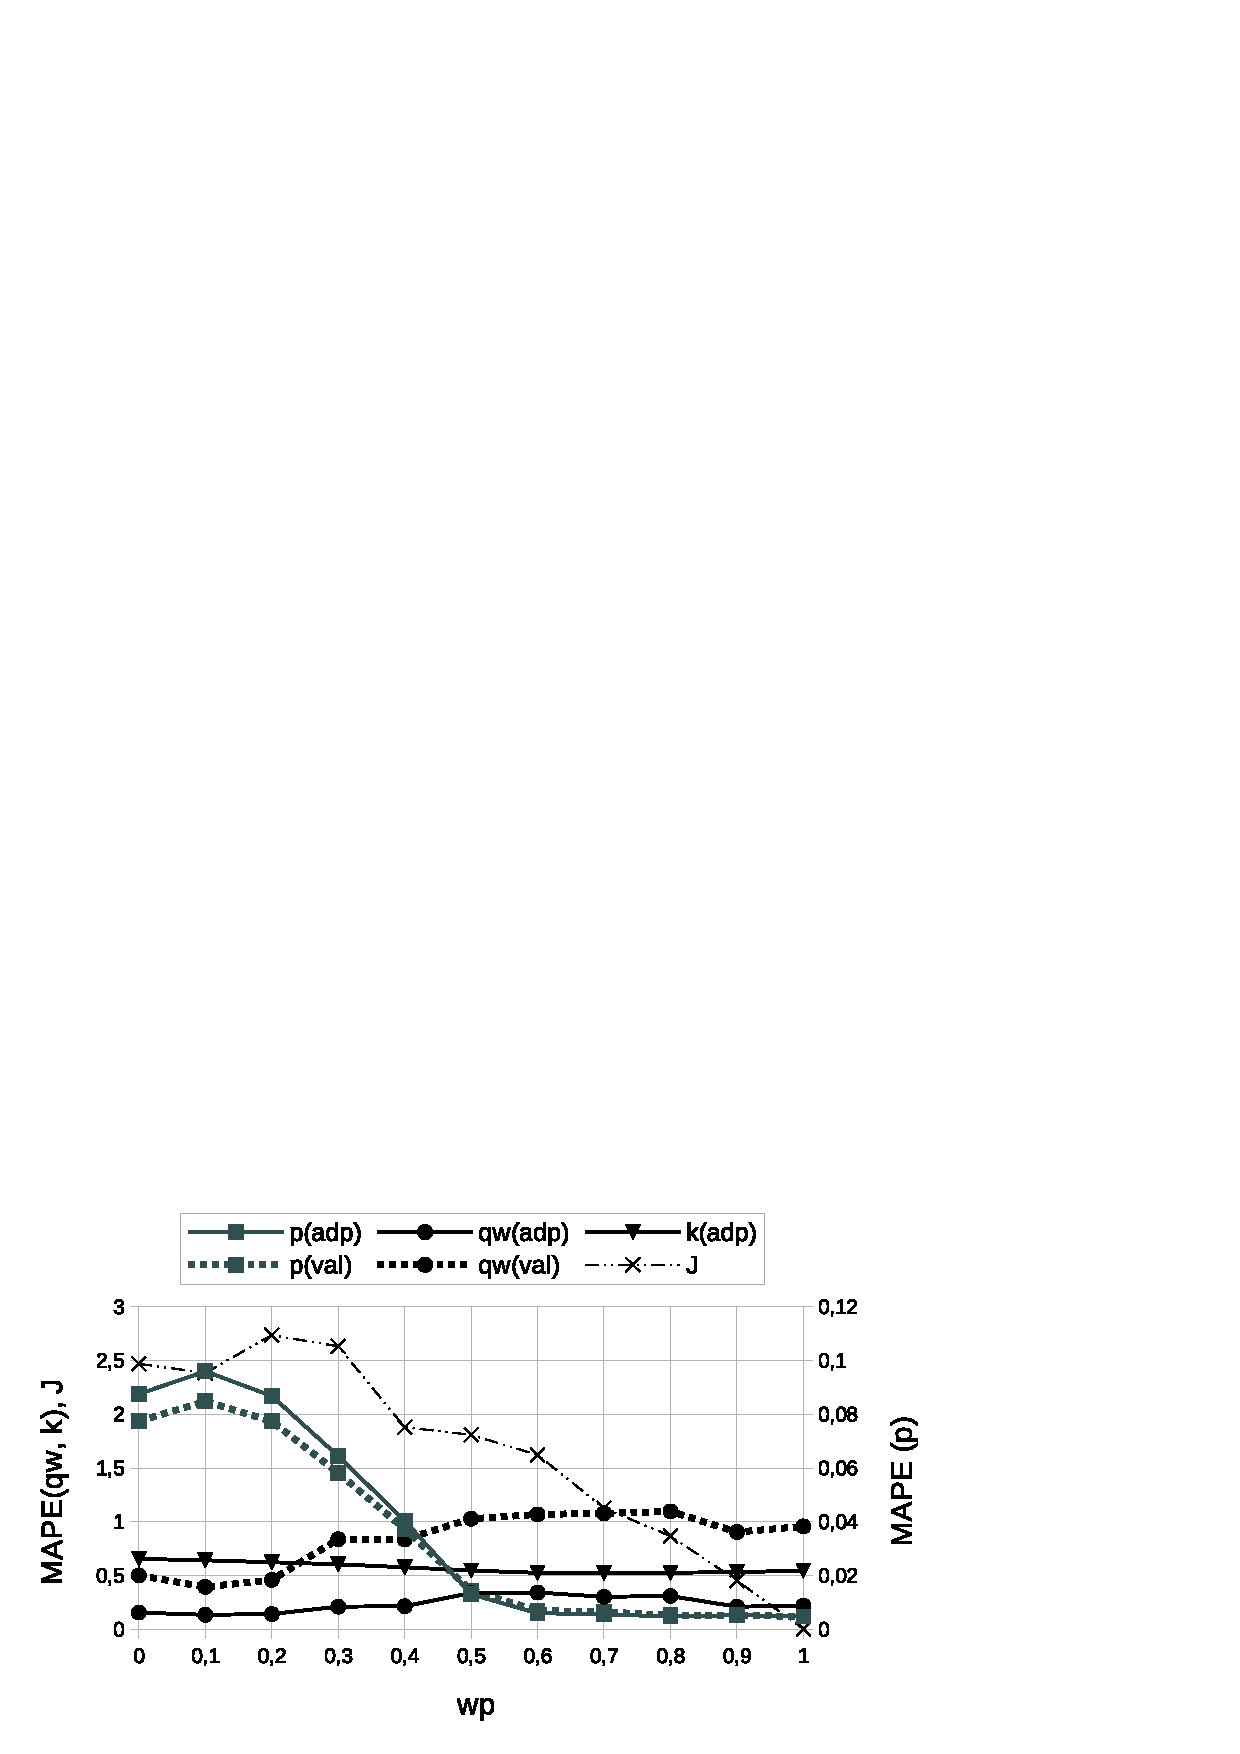
\includegraphics[height=0.60\linewidth]{fig4.png}}
		\caption{The reconstituted field of mobility}
		\label{fig:mob}
	\end{minipage} \hfill
	\begin{minipage}[h]{0.48\linewidth}
		\center{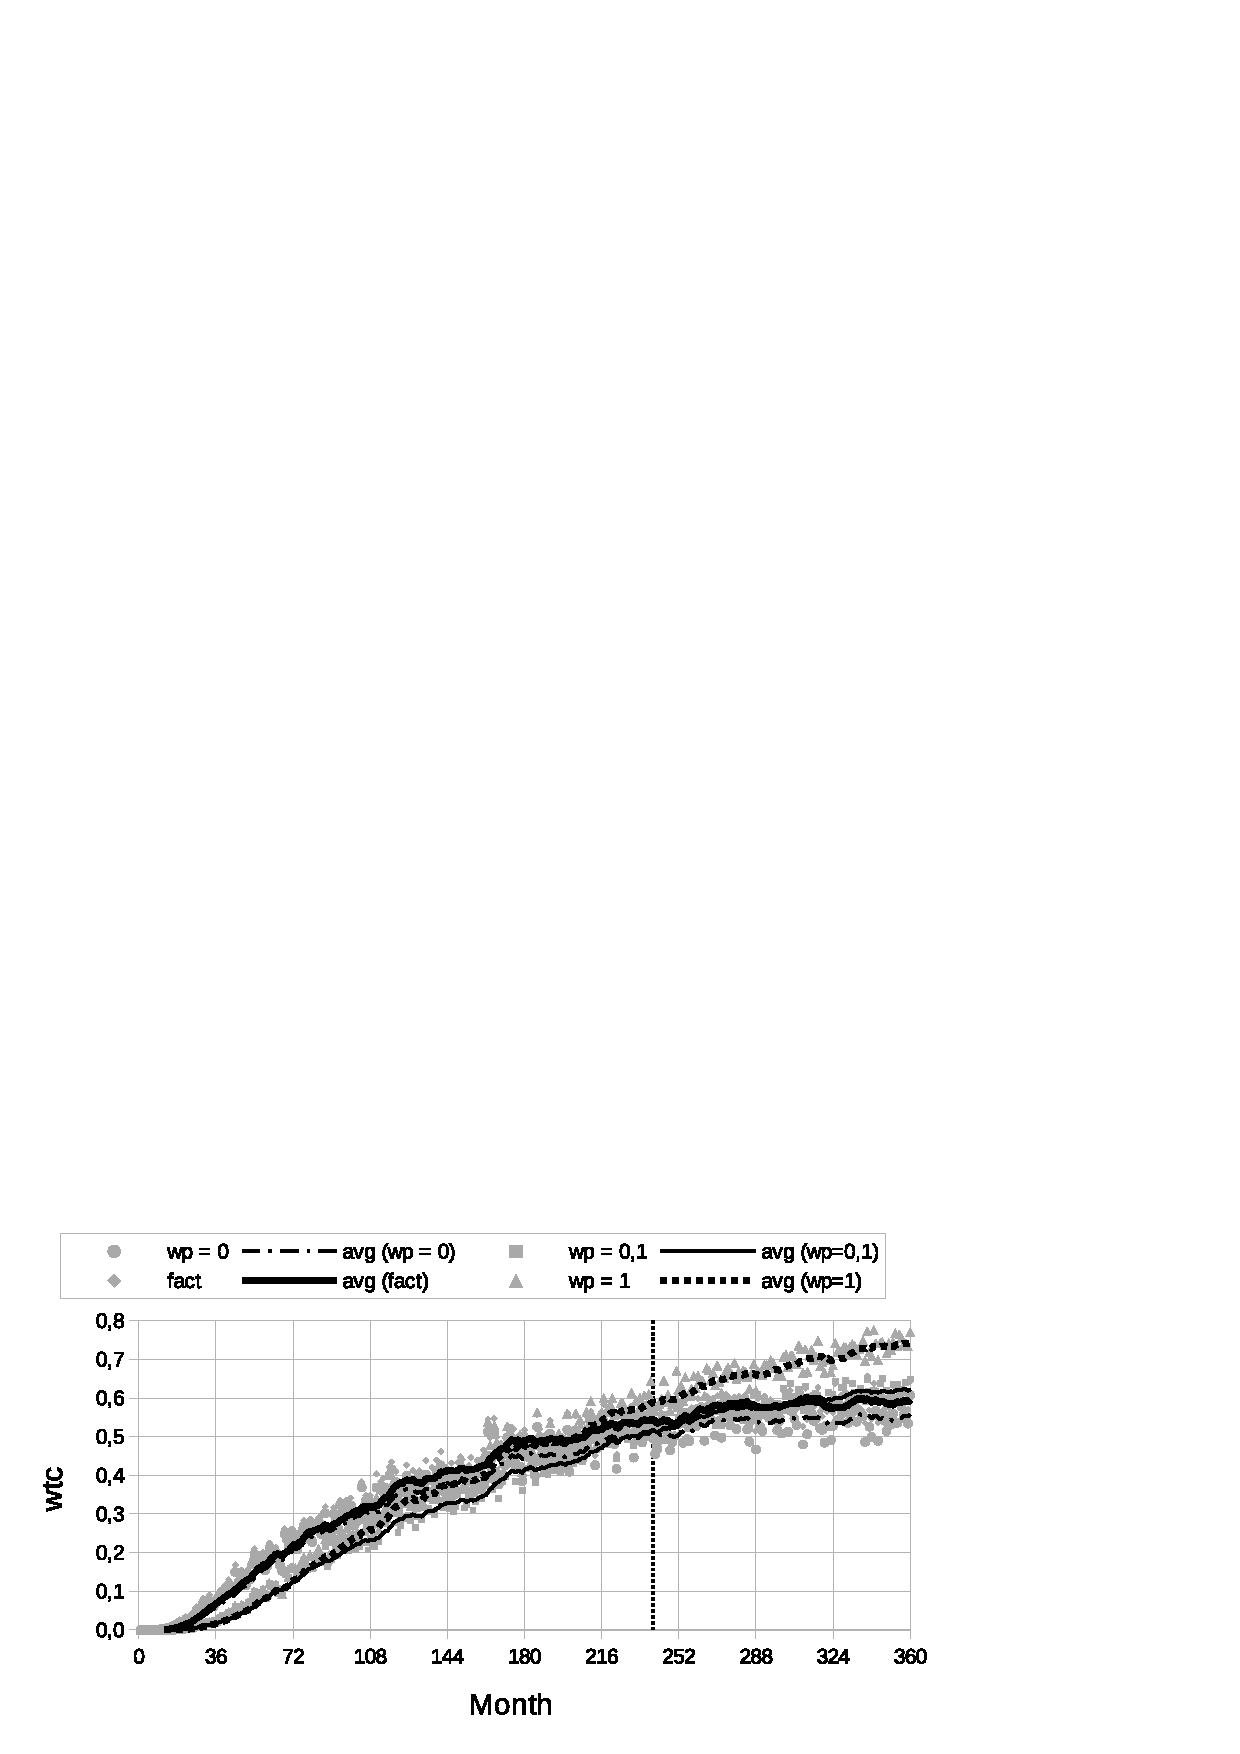
\includegraphics[height=0.60\linewidth]{fig5.png}}
		\caption{The restored compressibility field}
		\label{fig:comp}
	\end{minipage}
\end{figure}

A quantitative comparison between the actual and reconstructed fields of overall mobility was conducted based on the relationships derived from the values between wells. A comparison between the main links is provided in Table \ref{tabl:connection}, which demonstrates that the rank order of reconstructed links fully aligns with that of actual links. Additionally, a satisfactory level of quantitative agreement was achieved between the values of bonds: on average, the absolute error is 9\%. Therefore, the reconstructed field of overall mobility faithfully reproduces the key characteristics of the actual field both qualitatively and quantitatively.

\begin{figure}
	\centering
	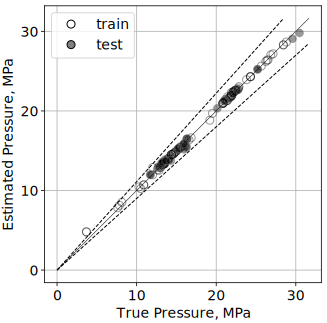
\includegraphics[width=0.7\linewidth]{fig6}
	\caption{Comparison of true and calculated values of reservoir pressure for production and injection wells. Hollow markers correspond to the training set, filled markers correspond to the test set. The dotted line indicates the 10\% deviation interval}
	\label{fig:cp}
\end{figure}

For real reservoir systems, the magnitude of the connections between wells is usually not reliably known. In view of this, one of the main criteria for assessing the quality of model adaptation is reservoir pressure measurements. In Fig. \ref{fig:cp} the comparison of the values of the actual and calculated pressures for a pair of wells I1, P1 obtained after the restoration of the field of general mobility and effective compressibility is given. In the figure, different markers indicate the values of the corresponding training (train) and test (test) samples. A satisfactory coincidence of pressures was obtained in the training and test samples, the values of the average relative error for which are 3.6 and 5.5\%, respectively. The model demonstrates satisfactory accuracy in the test sample, which confirms its predictive properties.



\begin{table}[h!]
	\caption{Coefficients of connections between wells}	
	\label{tabl:connection}	
	\begin{center}
		\begin{tabular}{c|c|c|c|c}
			\hline
			Connection & True value & Estimated  value & MAPE, \% \\
			\hline
			I2-P1 & 20.6 & 20.6 & 0.1 \\ 
			I3-P3 & 5.51 & 5.51 & 0.1 \\ 
			P3-I2 & 0.488 & 0.488 & 0.1 \\ 
			I1-P1 & 0.338 & 0.338 & 0.1 \\ 
			I4-P3 & 0.297 & 0.297 & 0.1 \\ 
			P3-I1 & 0.296 & 0.296 & 0.1 \\ 
			P5-I3 & 0.295 & 0.295 & 0.1 \\ 
			\hline
			
		\end{tabular}
	\end{center}
\end{table}

\section{CONCLUSIONS}

An approach to the combined use of filtering theory and machine learning has been developed in order to adapt a one-phase model to historical data. Using a synthetic model of an oil field element with a regionally inhomogeneous permeability field and effective compressibility as an example, the implementation of these approaches has been demonstrated. The adaptation of the one-phase filtration model to historical data was achieved by reconstructing the permeability and effective compressibility fields using a network of radial basis functions. Based on the reconstructed fields, the coupling coefficients between wells are calculated, which quantitatively correspond to true connections in the system.


\begin{acknowledgments}
The research was carried out at the expense of a grant from the Russian Science Foundation No. 24-21-00468,
https://rscf.ru/project/24-21-00468/�
\end{acknowledgments}

% Text of article ends here.

%
% The Bibliography
%

\begin{thebibliography}{99}
\bibitem{mus1}
\refitem{article}
 E. N. Musakaev, S. P. Rodionov and N. G. Musakaev, "Hierarchical Approach to Identifying Fluid Flow Models in a Heterogeneous Porous Medium," Mathematics, {\bf 9}(24), 3289 (2021).

\bibitem{bek}
\refitem{article}
 A. D. Bekman, T. A. Pospelova and D. V. Zelenin,  "A new approach to water cut forecasting based on results of capacitance resistance modeling" Vestn. Tyumen. Univ., Fiz. Mat. Model. Neft', Gaz, Energet. {\bf 6} (1(21)), 192--207 (2020).

\bibitem{pot}
\refitem{article}
 K.A. Potashev, R.R. Akhunov and  A.B. Mazo, "Calculation of the flow rate between wells in the flow model of an oil reservoir using streamlines", Georesources. {\bf 24}(1), 27--35 (2022).

\bibitem{tem}
\refitem{article}
P. Temirchev, M. Simonov, R. Kostoev, E. Burnaev, I. Oseledets, A. Akhmetov, A. Margarit, A. Sitnikov and D. Koroteev, "Deep neural networks predicting oil movement in a development unit", Journal of Petroleum Science and Engineering. 184. 106513 (2020).

\bibitem{uma}
\refitem{article}
A. W. Umanovskiy, "Proxy modeling pf reservoir hydrodynamics with graph neural networks",Vestn. Tyumen. Univ., Fiz. Mat. Model. Neft', Gaz, Energet. {\bf 8} (3(31)), 155--177 (2022).

\bibitem{kos2}
\refitem{article}
V. P. Kosyakov and D. Yu. Legostaev, "Using elements of machine learning to solve the inverse problem of reconstructing the hydraulic conductivity feld for a fltration problem", Vestn. Tyumen. Univ., Fiz. Mat. Model. Neft', Gaz, Energet. {\bf 8} (2 (30)), 129--149 (2022).

\bibitem{bas}
\refitem{book}
K. S. Basniev, N. M. Dmitriev, R. D. Kanevskaya, and V. M. Maksimov,  \textit{Underground Hydromechanics} (Inst.
Komp'yut. Issled., Moscow, 2006) [in Russian].


\bibitem{kos3}
\refitem{article}
V.P.Kosyakov, S.P.Rodionov, "Optimal control of wells on the basis of two-phase filtration equations",  Tr. MFTI. {\bf 8}(3), 79--90 (2016).

\bibitem{far}
\refitem{article}
P. E. Farrell, D. A. Ham, S. W. Funke and M. E. Rognes, "Automated Derivation of the Adjoint of High-Level Transient Finite Element Programs", SIAM Journal on Scientific Computing, {\bf 35}(4) 369--393 (2013).

\bibitem{inn}
\refitem{article}
M. Innes, E. Saba, K. Fischer, D. Gandhi, M. C. Rudilosso, N. M. Joy, T. Karmali, A. Pal and V. B. Shah, "Fashionable Modelling with Flux", ArXiv. 1811.01457 (2018).

\bibitem{and}
\refitem{book}
 V. B. Andreev, \textit{Numerical methods}. (M.: MAKS Press)[in Russian].

\bibitem{azi}
\refitem{book}
 H. Aziz, E. Settari, \textit{Mathematical modeling of reservoir systems},  M.-Izhevsk: Institute for Computer Research, 2004. [in Russian]

\end{thebibliography}
\end{document}
